%-----------------------------------------
% Lebenslauf Vorlage auf Deutsch
% Entworfen von Atefeh Aghababaei
% Sommer 2024
%-----------------------------------------
\documentclass[oneside]{article}

\usepackage{wallpaper}
\usepackage{geometry}
\usepackage[
    unicode=true,
    bookmarks=true,
    bookmarksnumbered=false,
    bookmarksopen=true,
    bookmarksopenlevel=1,
    breaklinks=false,
    pdfborder={0 0 0},
    backref=false,
    colorlinks=false
    ]{hyperref}
\usepackage{lastpage}
\usepackage{hyphenat}
\usepackage{hyphsubst}
\usepackage{tabularx}
\usepackage{moresize}
\usepackage[document]{ragged2e}
\usepackage[scaled]{helvet}
\usepackage{fontawesome5}
\usepackage[defaultfam,tabular,oldstyle]{montserrat}
\usepackage[T1]{fontenc}
\usepackage{titlesec}
\usepackage{xcolor}
\usepackage{tikz}
\renewcommand*\oldstylenums[1]{{\fontfamily{Montserrat-TOsF}\selectfont #1}}
\setlength{\parindent}{0pt}
\titleformat{\section}{\normalfont}{}{0pt}{}
\renewcommand{\arraystretch}{1.4}
\setlength\fboxrule{0pt}
\setlength\fboxsep{10pt}
\titlespacing{\section}{0pt}{1.5ex plus .1ex minus .2ex}{1pc}
\newcolumntype{Y}{>{\RaggedRight\arraybackslash}X}

%-----------------------------------------
%
%     Change PDF Meta Info here
%
%-----------------------------------------
\hypersetup{
    pdftitle={Atefeh Aghababaei - CV - English},
    pdfauthor={Atefeh Aghababaei},
    pdfsubject={CV}
}

% Paper size
\geometry{
    a4paper,
    left=0pt,
    right=20pt,
    top=0pt,
    bottom=0pt,
    nohead,
    % includefoot,
    nomarginpar
}

% Background Color of the Sidebar Column
\definecolor{sidebg}{cmyk}{0.17, 0.14, 0.14, 0.02}

% Background Color of the Main Column
\definecolor{mainbg}{cmyk}{0, 0, 0, 0}

% Text Color of the Main Column
\definecolor{maintext}{cmyk}{1, 0.02, 0, 0.8}

% Text Color of the Sidebar Column
\definecolor{sidetext}{cmyk}{1, 0.02, 0, 0.8}

\pagecolor{mainbg}

%-----------------------------------------

\begin{document}
\setlength{\topskip}{0pt}\setlength{\footskip}{0pt}%
\fcolorbox{red}{sidebg}{%
    \begin{minipage}[t][\textheight-2\fboxsep-2\fboxrule][t]{\dimexpr0.41\textwidth-2\fboxrule-2\fboxsep\relax}
        \color{sidetext}
        %-----------------------------------------
        % Persönliche Informationen
        %-----------------------------------------
        \begin{center}
            \begin{tikzpicture}
            \clip (0,0) circle (3.015cm) node[anchor=center] {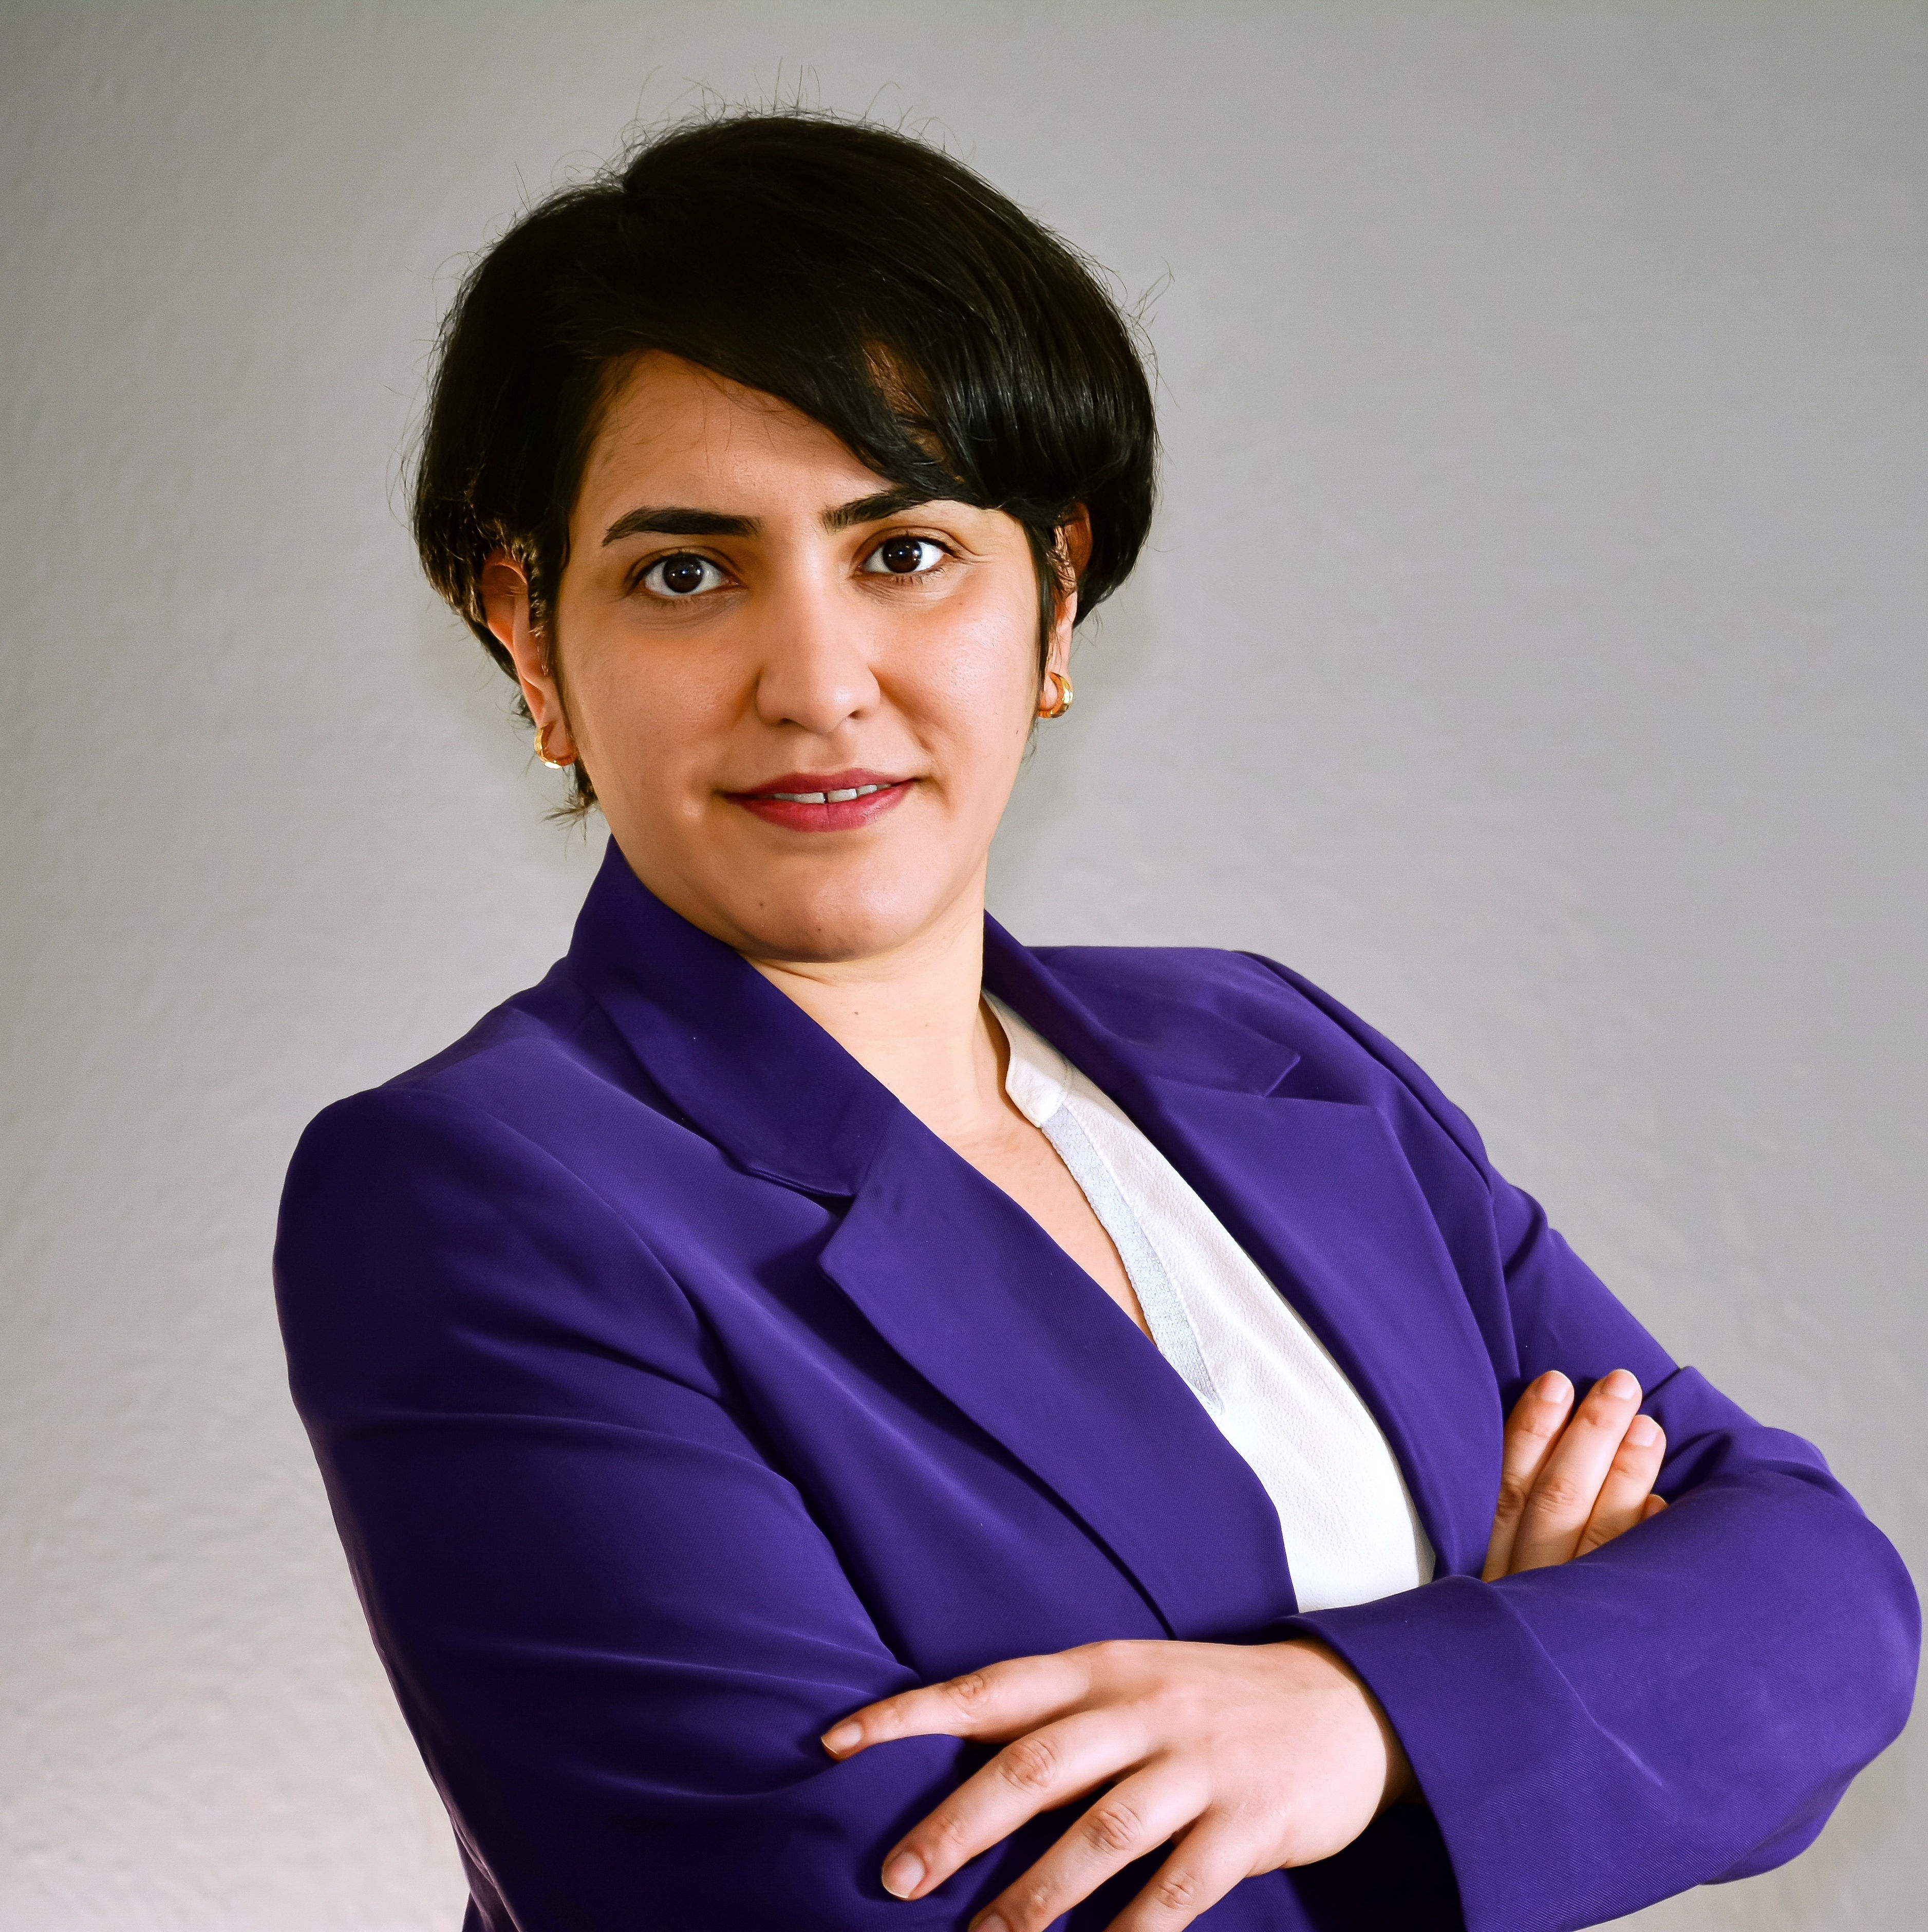
\includegraphics[width=6cm]{photos/business_foto.jpg}}; 
            \end{tikzpicture}
        \end{center}
        %\vspace{.3cm}
        {\bfseries Dr. rer. nat.} \\
        \vspace{.2cm}
        {\bfseries\huge Atefeh} \\
        \vspace{.2cm}
        {\bfseries\huge Aghababaei} %\qquad {they/them}
        \vspace{.2cm} \\
        Data Scientist 
        \vspace{7pt} \\
        %-----------------------------------------
        \rule{\linewidth}{0.4pt} \\
        \phantomsection{}
        \addcontentsline{toc}{section}{Kontakt}
        \section*{\large Kontakt}
        \begin{tabularx}{\textwidth}{@{}lX@{}} %{cY}
            %\faStarOfLife{} & 01/01/1970 \\
            \faPhone{}      & +49 177 4922042 \\
            \faEnvelope{}   & \href{mailto:atefehbabaei90@gmail.com}{atefehbabaei90@gmail.com} \\
            \faMapMarker{}  & {Paul-Schall\"uck Str. 21, 50939 K\"oln} \\
            \faLinkedin{} & \href{https://www.linkedin.com/in/atefeh-babaei/}{/atefeh-babaei} \\
            \faXing{}     & \href{https://www.xing.com/profile/AtefehMitra_Aghababaei}{/AtefehMitra\_Aghababaei} \\
        \end{tabularx}
        \vspace{4pt} \\
        \rule{\linewidth}{0.4pt} \\
        %-----------------------------------------
        \phantomsection{}
        \addcontentsline{toc}{section}{Pers\"onliche Daten}
        \section*{\large Pers\"onliche Daten}
        \begin{tabularx}{\textwidth}{@{}lX@{}} %{cY}
            %\faStarOfLife{} & Geburtsdatum: 17/05/1990 \\
            \faFlag{}      & \textbf{\small Staatsangeh\"origkeit}:\newline Deutsch $\bullet$ Iranisch \\
            
        \end{tabularx}
        \vspace{2pt} \\
        \rule{\linewidth}{0.4pt} \\
        %-----------------------------------------
        % FÄHIGKEITEN (Skills)
        %-----------------------------------------
        \phantomsection{}
        \addcontentsline{toc}{section}{Kompetenzen}
        \section*{\large Kompetenzen}

        \begin{tabularx}{\textwidth}{@{}lX@{}} % Adjusted for no extra space at start and end of table
            \faLanguage{}   & \textbf{\small Sprachen:} \newline  Persisch (Muttersprache) \newline Englisch (Verhandlungssicher) \newline Deutsch (Flie\ss end).\\
            \faCode{}        & \textbf{\small Programmiersprachen:} \newline Python $\bullet$ SQL $\bullet$ Bash $\bullet$  R $\bullet$ MATLAB.\\
            
            \faLaptopCode{}  & \textbf{\small Bibliotheken:} \newline Pandas $\bullet$ Matplotlib $\bullet$  NumPy $\bullet$ SciPy $\bullet$ Scikit-learn $\bullet$ PyTorch $\bullet$ Jupyter. \\
            
            \faCogs{}        & \textbf{\small Sonstige Methoden:} \newline Statistische Methoden $\bullet$ Big Data $\bullet$ Datenanalyse $\bullet$ Datenvisualisierung $\bullet$ Bildverarbeitung $\bullet$ Fehlerbehebung $\bullet$ Data Mining $\bullet$ Datenmanagement $\bullet$ Maschinelles Lernen $\bullet$ Git. \\ % Maschinelles Lernen 
            
            \faToolbox{}     & \textbf{\small Project Management:} \newline Agile Methodologien $\bullet$ Scrum $\bullet$ \newline Projektplanung $\bullet$ Confluence $\bullet$ Jira. \\
            
            \faCloud{}       & \textbf{\small Cloud Computing:}  \newline Grundlagen des Cloud Computing.% $\bullet$ Google Cloud. 
            \\
            
        \end{tabularx}


        \vspace{1pt}
        
    \end{minipage}
}
\hfill
\fcolorbox{red}{mainbg}{%
    \begin{minipage}[t][\dimexpr\textheight-2\fboxrule-2\fboxsep\relax][t]{\dimexpr0.60\textwidth-2\fboxrule-2\fboxsep\relax}
        \color{maintext}
        \vspace{17pt}
        {\justify \footnotesize Data Scientist und promovierte Physikerin mit \"uber sechs Jahre Erfahrung in der Entwicklung von Python-Tools zur Analyse und Visualisieren Datens\"atze. Meine St\"arke liegt darin, komplexe Fragestellungen durch das Entwickeln oder Anpassen agiler Methoden zu bew\"altigen, sowie Projekte mit einem Fokus auf die F\"orderung von Teamgeist zu leiten.
        }
        %-----------------------------------------
        % Berufserfahrung (WORK EXPERIENCE)
        %-----------------------------------------
        \phantomsection{}
        \addcontentsline{toc}{section}{Berufserfahrung}
        \section*{\scshape\Large Berufserfahrung \rule{\linewidth}{0.4pt}}
        \noindent
        {\large \textbf{Wissenschaftliche Mitarbeiterin}} \\ 
        {\scshape\fontseries{light}\selectfont\footnotesize Universit\"at zu K\"oln \qquad Mai. 2017 \textendash{} Sep. 2023} \\
        
        \begin{itemize}
            \setlength{\itemsep}{-3pt}
            \footnotesize
            \item Entwicklung von Python-Pipelines f\"ur die Analyse von Big Data.
            \item Ver\"offentlichungen in astronomischen Fachzeitschriften; Vortr\"age auf internationalen Konferenzen.
            \item Aufbau von weltweiten wissenschaftlichen Kooperationen.
            \item Betreuung von Master- und Bachelor-Studenten.
            \item Tutorin in vier Vorlesungen auf Master- und Bachelor-Niveau.
            \item Mitglied des Sonderförderungsbereich SFB-956 (F\"orderung durch DFG).
        \end{itemize}
        %-----------------------------------------
        {\large \textbf{Wissenschaftliche Hilfskraft}} \\
        {\scshape\fontseries{light}\selectfont\footnotesize Max-Planck-Institut f\"ur Radioastronomie (MPIFR) \qquad Mai 2014 \textendash{} Mai 2016} \\
        \begin{itemize}
            \setlength{\itemsep}{-3pt}
            \footnotesize
            \item Datenmanagement im VLBI-Data-Center.
            \item Bewertung der Phasierung von Datens\"atzen ALMA-Regressionstests.
            \item Kalibrierung und Visualisierung von Teleskop-Stichprobendatens\"atzen.
            \item Vergleich verschiedener Kalibrierungsmethoden f\"ur Datens\"atze \"uber verschiedene Radioteleskope hinweg.
        \end{itemize}
        %-----------------------------------------
        % Ausbildung (EDUCATION)
        %-----------------------------------------
        \phantomsection{}
        \addcontentsline{toc}{section}{Akademische Ausbildung}
        \section*{\scshape\Large Akademische Ausbildung \rule{\linewidth}{0.4pt}}
        \noindent
        {\large \textbf{Promotionsstudium \textendash{} Physik }} \\
        {\scshape\fontseries{light}\selectfont\footnotesize an der Universit\"at zu K\"oln \qquad Feb 2019 \textendash{} Oct. 2023} \\
        {\footnotesize Titel: Dr. rer. nat.} \\%[1ex]
        {\footnotesize Bereich: Experimentalphysik / Astrophysik} \\
        {\footnotesize Thema: Kinematics and Structure of Massive Star Formation in NGC6334-V} \\[2ex]
        {\large \textbf{Masterstudium \textendash{} Physik}} \\
        {\scshape\fontseries{light}\selectfont\footnotesize Bonn\textendash{}Cologne Graduate School \qquad Apr 2016 \textendash{} Aug 2018} \\
        {\footnotesize Bereich: Experimentalphysik / Astrophysik} \\
        {\footnotesize Masterarbeit: Characterizing the High Mass Protocluster NGC6334-V via High-Resolution ALMA Observations} \\
        %-----------------------------------------
        % Zertifikate (Certifications)
        %-----------------------------------------
        \phantomsection{}
        \addcontentsline{toc}{section}{Zertifikate}
        \section*{\scshape\Large Zertifikate \rule{\linewidth}{0.4pt}}
        \noindent
        {\textbf{SQL}}\newline { \footnotesize SQLite Essential Training}\\[1ex]
        {\textbf{Projektmanagement-Grundlagen}}\newline{ \footnotesize Ethik $\bullet$ Anforderungen $\bullet$ Zeitpläne $\bullet$ Budgets $\bullet$ Teams $\bullet$ Kommunikation $\bullet$ Risiko $\bullet$ Stakeholder}\\[1ex]
        {\textbf{Cloud-Konzepte}}\newline { \footnotesize Cloud-Architektur $\bullet$ Cloud Computing $\bullet$ Cloud-Sicherheit $\bullet$ Bestimmung der Cloud-Strategie $\bullet$ IBM Certified Cloud Professional Architect}
        %-----------------------------------------
        % Voluntary Activities
        %-----------------------------------------
        \phantomsection{}
        \addcontentsline{toc}{section}{Z\"uzastliche T\"atigkeiten}
        \section*{\scshape\Large Z\"uzastliche T\"atigkeiten \rule{\linewidth}{0.4pt}}
        
        \noindent
        {\textbf{Erste Sprecherin und Hauptmitglied} \newline \footnotesize  Sonderforschungsbereich (SFB 956) Studentenrat} \\
        {\scshape\fontseries{light}\selectfont\footnotesize Universität zu Köln \qquad Jun. 2019 \textendash{} Nov. 2021} \\[1ex]

        {\textbf{Mitglied des Organisationskomitee} \newline \footnotesize  Assembly of the European Astronomical Society (EAS)} \\
        {\scshape\fontseries{light}\selectfont\footnotesize Leiden (Virtuell) \qquad Jun 2021 \textendash{} Jul. 2021} \\[1ex]
        
        {\textbf{Mitglied des Organisationskomitee} \newline \footnotesize  30th General Assembly of the International Astronomical Union (IAU)} \\
        {\scshape\fontseries{light}\selectfont\footnotesize Wien \qquad Aug. 2018 } \\

        %-----------------------------------------

        \vspace{15pt}

        \noindent
        \begin{minipage}[c]{0.97\textwidth} 
        \flushright
        \footnotesize K\"oln, \qquad \today \\
        \footnotesize Dr. Atefeh Aghababaei
        \end{minipage}%
        \hfill
        
    \end{minipage}
}%


\end{document}